\documentclass[A4paper,11pt]{article}

\usepackage{latexsym}
\usepackage{epsfig}
\usepackage{verbatim}
\usepackage{shadow}
\usepackage{amssymb}
\usepackage{amsmath}
\usepackage{graphicx}
\usepackage{color}
\usepackage{bm}
\usepackage{fancyhdr}

\addtolength{\textwidth}{4cm}
\addtolength{\textheight}{6.5cm}
\addtolength{\oddsidemargin}{-2cm}
\addtolength{\topmargin}{-4.5cm}

\newtheorem{theorem}{\sc Theorem}[section]
\newtheorem{lemma}[theorem]{\sc Lemma}
\newtheorem{corollary}[theorem]{\sc Corollary}
\newtheorem{fact}[theorem]{\sc Fact}
\newtheorem{remark}[theorem]{\sc Remark}

\author{
	{\sc Guangyu Dong} \\
	\texttt{gdong2@illinois.edu}
	\and
	{\sc Randall Hill} \\
	\texttt{rwhill2@illinois.edu}
	\and
	{\sc Vasileios Livanos} \\
	\texttt{livanos3@illinois.edu}
}

\title{
Resource-Constrained Prospect Theory
}

\date{}

\begin{document} \maketitle

\par Consider $n$ agents, numbered $1$ through $n$, interacting in a social network. We represent this social network as
an undirected weighted graph $G = (V, E)$, where $V = \{ 1, 2, \cdots, n \}$ represents the agents and $E$ represents
for each agent the set of agents she is interacting with. The weight of an edge $\{ i, j \} \in E$ denotes the frequency of
interaction between agents $i$ and $j$, and we also denote the neighborhood of an agent $i$ by
$\mathcal{N}_i = \big\{ j \: | \: \{ i, j \} \in E \big\}$.

\par In this network, each agent has a set of strategies available to her. Specifically, agent $i$ proposes an
interaction frequency $f_{ij} \in \mathbb{R}$ to every agent $j \in \mathcal{N}_i$. Similarly, each agent $j$ proposes an
interaction frequency $f_{ji}$ to $i$. The frequency that they end up interacting at is simply the minimum of the two
proposals. However, in real social networks, the agents have different preferences for who to interact with. To capture this
in our model, we assign $w_{ij}$ to be the weight $i$ places on $j$, or similarly how much $i$ values the interaction with $j$.
Further motivated by real social networks, we assign all agents a uniform ``budget" of interaction frequency $\beta$ that they
cannot exceed.

\par In our model we deviate from standard practices in algorithmic game theory and instead of considering that agents act
in accordance with the predictions of the expected utility theory, we consider the case where the behavior of the network's
agents is better captured by prospect theory. Prospect theory, introduced by Kahneman and Tversky \cite{KT}, states that people
make decisions based on the potential value of losses and gains rather than the final outcome, and that people evaluate these
losses and gains using certain heuristics. This model attempts to depict real-life scenarios, where the agents sometimes act
irrationally rather than making the optimal decisions for them. Therefore, we consider utility functions that capture the
observation of prospect theory that in real-life situations people are loss-averse; in mathematical terms, if $u_i(x)$ is the
utility of player $i$ with $x$ being the strategy profile, then $- u_i(-x) > u(x)$. In other words, utility functions studied
by prospect theory are similar to the one in Figure \ref{fig:prospect-util}, with the curve for losses being ``steeper" than
the curve for gains.

\begin{figure}[h!]
  \centering
  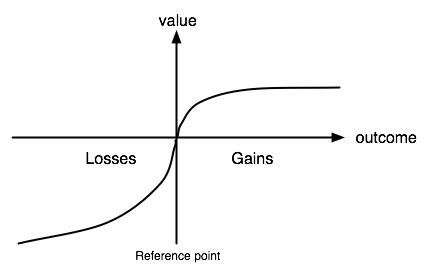
\includegraphics[width=.35\linewidth]{./Valuefun.jpg}
  \caption{An agent's utility function as described by prospect theory}
  \label{fig:prospect-util}
\end{figure}

\par It is clear that our approach is motivated by real-life social networks therefore an analysis would not be complete
if it remained in a theoretical level. To this end, we gather data from real online social networks (i.e. Twitter) in
order to understand whether the observations from real social networks are similar to the predictions of our model.

\label{Bibliography}

\lhead{\emph{Bibliography}}

\bibliographystyle{abbrv}

\bibliography{one-pager} % The references (bibliography) information are stored in the file named "Bibliography.bib"

\end{document}
